\chapter{Search}
We will go over \textbf{uninformed} (given no information except problem definition) and \textbf{informed} search (given some guidance on where solutions are) algorithms. 

\section{Problem solving agents}
We need to formulate the problem first by deciding what actions and states to consider, given a goal. Process of looking for a sequence of actions to reach goal is called \textbf{search}. 

An \textbf{incremental formulation} starts with the empty state and adds each state incrementally. A \textbf{complete-state formulation}  starts with the set of things that can be on and then tries to optimize them.


\section{Searching}
We start at the root node. We then expand the current state, so the branches of the current node we are at. Then we choose which of these three children to consider. Each child is called a \textbf{leaf node}  and set of all leaf nodes to be expanded is called a \textbf{frontier}.


Some graphs have loopy paths such that one ends up traversing a loop in the graph indefinitely.

The general approach to a graph search algorithm is, 

\begin{verbatim}
func GRAPH-SEARCH(problem) returns solution,failure
    init frontier with initial state
    init explored set as empty
    loop do
        if frontier empty return with failure
        choose leaf node, remove from frontier
        if node is goal return solution
        add node to explored set
        expand node
            if children not in explored add to frontier
\end{verbatim}

\subsection{Measuring performance}
\begin{itemize}
    \item \textbf{Completeness}: Is the also guaranteed to find solution if it exists 
    \item \textbf{Optimality}: Does it find the optimal solution
    \item \textbf{Time complexity}: How long to find solution
    \item \textbf{Space Complexity}: How much memory is required
\end{itemize}

b, \textbf{branching factor}  is the max num of successors of any node and d, \textbf{depth}  is the depth of the shallowest goal and m, is the \textbf{max length} of any path in the state space.

\section{Uninformed Search}
\subsection{Breadth-first search}
Root node is expanded first, all successors are next and their successors. So all nodes expanded at a given depth before we go on to the next level.

Need a \textbf{FIFO }(first in first out) queue.

Metrics are, 
\begin{itemize}
    \item Complete: Yes. If the goal is in some finite depth, BFS will eventually reach it.
    \item Optimal: No. Shallowest goal is not necessarily the most optimal
    \item Time Complexity: At depth d we will have $b^{d}$ nodes so we have,
        $$ b + \dots + b^{d} = O(b^{d}) $$ 
    \item Space complexity: We store every expanded in explored. So we have $O(b^{d - 1})$ nodes in the explored and $O(b^{d})$ in the frontier. Latter dominates so that is the space complexity.
\end{itemize}


Main problems are memory requirements. 


\subsection*{Uniform-cost search}
Is optimal with any step-cost function. Instead of expanding the shallowest node, UCS expands the node with the lowest path cost $g(n)$. Stores frontier as a priority queue (heap).

The goal test on a node is when we expand the node and not when we add it to the frontier. Because when we add we may be on a sub optimal path and a better path may exist in the current frontier.
\begin{itemize}
    \item Complete: Yes if provided cost is non-zero, if not it can get stuck in an infinite loop.
    \item Optimal: Yes. Optimal in general.
    \item Time Complexity: Worse than breadth search. If all cost is same it is equivalent to breadth in terms of function however even if it finds the goal node as it expands all of its children its $b^{d + 1}$
\end{itemize}

\subsection{Depth-first search}
Expands deepest node in frontier. Basically deepest level until nodes have no children. Then goes one up to next deepest node with unexplored successors and so on. Uses a \textbf{LIFO }queue or a \textbf{STACK}.

Generally implemented using a recursive function. 



\begin{itemize}
    \item Complete: In finite state space if Graph-search is used its complete (as we have explored set to prevent loops). If Tree-search is used its not complete. However in finite state space both fail.
    \item Optimal: Both versions are non-optimal
    \item Time Complexity: Depends on state space. We have $O(b^{m})$ where $m$ is the max depth. Can be greater than the state space itself (if finite).
\end{itemize}

Depth-first only advantage is its space complexity which is $O(bm)$ as you don't need to store all children. Can delete if a node has been expanded, can be removed after all its children are explored.

\textbf{Backtracking search} is a variant uses less memory. Only one successor is generated at a time than all successors. Each partially expanded node knows what to expand next.


\subsection{Depth-limited search}
We limit the depth to $l$. Assume nodes at level $l$ have no children. Is obviously incomplete as if goal exists at level $> l$ it won't be found.

\subsection{Iterative deepening depth-first search}
Iteratively increase the limit - first 0, then 1,2, \dots until goal is found. Combines benefit for DFS and BFS searches. Makes it complete. Space complexity is $\mathbf{O(bd)}$. Time complexity is  $\mathbf{O(b^{d})} $

Is the preferred uninformed search algo.

\subsection{Bidirectional search}
We run two simultaneous searches - from forward from initial state and backward from goal. Motivation is $b^{d /2} + b^{d /2}$ is better than $b^{d}$. 

Search ends when frontiers of the two searches intersect (The first sol might not be the most optimal). Additional search required. 



\begin{itemize}
    \item Complete: Is complete
    \item Optimal: Depends on stopping condition.
    \item Time Complexity: $O(b^{\frac{d}{2}})$
\end{itemize}


\subsection{Summary of uninformed search strategies}

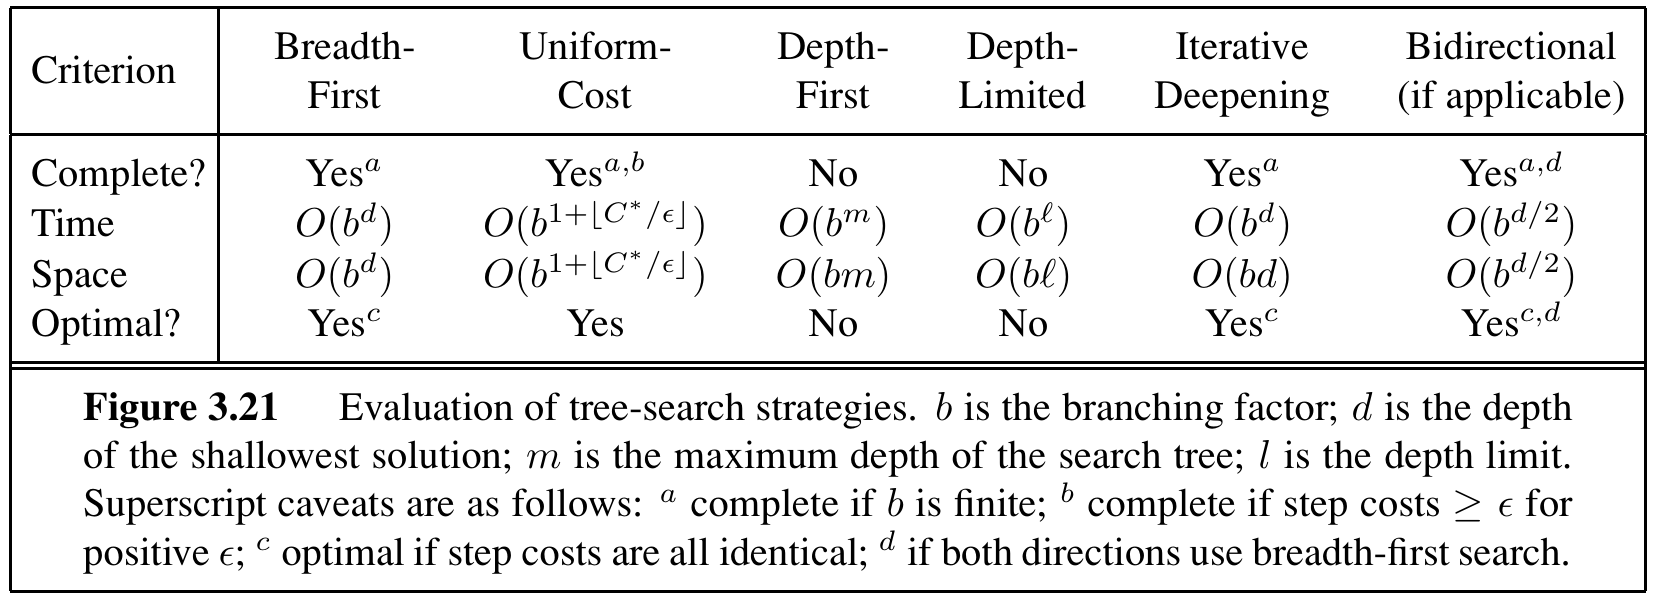
\includegraphics[width=\textwidth]{uninformed_search}


\section{Informed (Heuristic) Search}
Uses problem-specific knowledge beyond definition of problem - more efficient than uninformed.

General approach - \textbf{best-first search}. Node is selected based on an \textbf{evaluation function} $f(n)$ ( a cost estimate). So node with lowest  $f(n)$ is chosen.  Choice of $f$ determines the search strategy. $h(n)$ is the heuristic function which is a part of $f(n)$.

\begin{center}
$h(n)$ = estimated cost of the cheapest path from $n$ to a goal.
\end{center}

$h(n)$ is similar to $g(n)$ but $h(n)$ is dependent on the state and not the path. For instance one node in UCS might have different $g(n)$ depending on the path it takes. However it can only have the same  $h(n)$.

\subsection{Greedy best-first}
Expands the node closest to the goal. So $f(n) = h(n)$. Eg. for maps our  $h(n)$ can just be the straight line distance from node to goal. It is not optimal - rather greedy.

Graph version is complete in finite spaces but not in infinite, tree is not complete (can be stuck in loops). Space and time complexity are $O(b^{m})$ where m is max depth. Different heuristics can make it better.

\subsection{A* search}
Our evaluation function is, 
$$ f(n) = g(n) + h(n) $$ 
Where $g(n)$ is path cost from start node to $n$ and $h(n)$ is cost of cheapest path from $n$ to goal.

So we try the node with lowest $g(n) + h(n)$. Works only if $h(n)$ satisfies certain conditions. It is both \textbf{Complete and Optimal}

\subsubsection{Conditions for optimality}
\begin{itemize}
    \item $h(n)$ needs to be a \textbf{admissible heuristic}: One that never overestimates the cost to reach the goal.  Here $g(n)$ is the actual cost till current node. So if $h(n)$ overestimates then $f(n)$ overestimates. If this happens then good paths could never be explored (non-optimal).
    \item $h(n)$ needs to be \textbf{consistent} (relevant for graph search only): For every node $n$ and every successor $n'$ of n generated by action $a$, the estimated cost of reaching the goal from $n$ is no greater than the step cost of getting to $n'$ plus the estimated cost of reaching goal from $n'$.
    $$ h(n) \le c(n,a,n') + h(n') $$ 
\end{itemize}

\subsubsection{Optimality of A*}
The tree search version is optimal if $h(n)$ is admissible and the graph search is optimal if $h(n)$ is consistent.

If $h(n)$ is consistent then the values of $f(n)$ along any path is non decreasing, 
$$ f(n) \le f(n') $$ 


$A*$ is \textbf{optimally efficient} for any given consistent heuristic. No other optimal algo is guaranteed to expand fewer nodes than $A^{*}$ because $A^{*}$ expands all nodes with $f(n) < C^{*}$ where $C^{*}$ is true cost of the optimal solution.

So $A^{*}$ is \textbf{complete, optimal and optimally efficient}  among all such algorithms.



